\documentclass[12pt, titlepage]{article}
\usepackage[utf8]{inputenc}
\usepackage{amssymb}
\usepackage{amsmath}
\usepackage{array}
\usepackage{booktabs,tabularx}
\usepackage{breqn}
\usepackage[utf8]{inputenc}
\usepackage{csquotes}
\usepackage{graphicx}
\usepackage{enumitem}
\usepackage[letterpaper,bindingoffset=0in,%
            left=1in,right=1in,top=1in,bottom=1in,%
            footskip=.25in]{geometry}
\usepackage{latexsym}
\usepackage{lipsum}
\usepackage{pgfplots}
\usepackage{pxfonts}
\usepackage[input-decimal-markers=.]{siunitx}
\usepackage{setspace}
\doublespacing
\usepackage{hyperref}
\hypersetup{
    colorlinks=true,
    linkcolor=magenta,
    filecolor=blue,
    urlcolor=magenta,
}

\title{Topic Modeling and Lyric Classification}
\author{Alan Chen and Mac Tan}
\date{December 2018}

\begin{document}
\maketitle

\section{Background}
Ask someone what kind of music they like and---if they don't start by naming artists---they'll invariably make a reference to some kind of genre: "I'm into old-school hip-hop" or "I'm a big classic rock fan" and other similar statements are common refrains. Genre is perhaps the key way people group and organize music. But how does the deaf community experience music? Do they have separate and/or distinctive interpretations of genres as typically defined by hearing people?

There is a dearth of research on the meaning and cultural impact of music in the deaf community (see Darrow 2006 for a rare example) \cite{darrow_2006}. But a 1993 ethnographic study revealed that singing songs was one of the most enjoyed musical activities among deaf individuals who involved themselves with music (Darrow 1993) \cite{darrow_1993}. In recent years music concert interpreters have become increasingly innovative in translating song lyrics into American Sign Language, in a manner more evocative of the emotional and rhythmic qualities of song (Caswell 2017) \cite{vox_2017}.

Given the emphasis on lyrics in music to the deaf community, we aim to evaluate if lyrics can classify musical genres. The performance of lyrical features in genre classification could be suggestive of whether or not the deaf community has a separate appreciation and interpretation of musical genres compared to those who are not deaf.

However, pinpointing exactly what constitutes genre is complex and circuitous. The best definition the Oxford Music Online encyclopedia is able to muster is genre as "a pairing of (socially and historically produced) conventions and expectations" which at least partly comprise stylistic archetypes and "codify past repetitions and invite future repetitions" (Samson, 2001) \cite{samson_2001}. Thus irregardless of hearing ability, music genres are not clearly defined, yet there is still clearly common ground for many songs as to which genre(s) a song does or does not belong to.

Given this, we hypothesize that there is a relationship between song genres and song lyrics. There is prior work on classifying songs using lyrics, such as that by Mayer et al. (2011) and by Logan et al. (2004) However, Mayer et al. use auditory data in conjunction with lyrics to accurately classify songs by genre using a support vector machine (678-679) \cite{mayer_2011}, while Logan et al. fail to achieve good classification performance on lyrics alone, possibly due to a small sample size. \cite{logan_2004} We conceive songs with lyrics as a collection of words, among other auditory characteristics, and as such we use topic modeling to characterize songs by specific distributions of words. This allows us to use these song-topic distributions as features to classify song genres. The success of these features in genre classification could shed light on whether the text characteristics of songs provide the same information about song genres as the other auditory characteristics do. Furthermore, the average association of genres to topics could suggest whether or not the deaf community may have a different experience with music compared to those who are not deaf.

\section{Methods}
All data analysis was run on R 3.4.2. We first use a topic model as a feature extraction method to predict song genres and inspect how well the recovered topics for each song align with the song's genre(s). After converting our corpus of song lyrics to a document-term matrix, we built topic models using latent Dirichlet allocation (LDA), an algorithm proposed by Blei, Ng, and Jordan (2003). \cite{blei} The LDA model assumes that a set number of topics probabilistically generates terms (words, ngrams), which together comprise a document. \cite{blei_2002} Using a Bayesian three-level hierarchical model, LDA is able to estimate the mixture of topics which comprise a document, and the mixture of terms that comprise the topics. In our implementation, documents are songs, and terms are individual words.

After fitting the LDA model on the entire corpus using the \texttt{topicmodels} library, we used the model to make predicted posterior probabilities for topic distributions for each song in the test set. These posterior probabilities effectively represent the mixture of topics covered by each song in the test set. Since there isn't a universally accepted way to

\begin{center}
    \includegraphics[width=7in]{lda_song_ngram1_k4.png}
\end{center}

\noindent determine the number of topics before fitting the LDA models, we began with LDA models set to 2, 4, 6, and 8 topics, respectively. 

The figure above shows the word distribution spread for the $k=4$ LDA model. Examining the top 15 words most likely to be generated by each topic, one topic is non-English entirely, one topic includes many words overwhelmingly common in hip-hop lyrics, and the remaining two are somewhat hard-to-differentiate sets of English words.

The other models fitted to fewer than 10 topics similarly showed topics that were either too broad and vague, or too specific to language and specifically the hip-hop genre. Because of the lack of variability in the topic-term distributions, we proceeded to fit LDA models with 10, 20, 30, 40, and 50 topics, respectively. We then used these posterior probabilities as features in a logistic model that predicts song genre, evaluating the model's performance on a test set. For simplicity and interpretability, we use logistic regression, even though other methods may perform better.

Effectively, we are using the LDA topic models as a dimension reduction method, capturing in relatively few topics the semantic information embedded in a large set of words. If our topics are able to do this well and accurately predict song genre, that suggests that the lyrical content of songs captures genre-specific semantic idiosyncrasies. Therefore, if we can use the LDA-generated posterior probabilities to predict genre well, we can infer that lyrics are enough to determine which genre(s) a song fits into. Consequently, members of the deaf community who engage with music may have similar understandings of musical genre classifications as those who are not hearing impaired.

\section{Data}
\subsection{Data sources}
To collect the data, we used the \texttt{httr}, \texttt{rvest}, and \texttt{xml2} libraries to scrape lyrics and metadata (artist, album, genre, release year) for 377,497 songs from the lyrics website \href{https://www.lyrics.com/}{Lyrics.com}, part of the \href{https://www.lyrics.com/about.php}{STANDS4 Network}. These songs constitute about 31\% of the more than 1.2 million songs available on the website. Our scraping methodology did not allow us to target specific genres, artists, or years and is thus a non-representative, albeit randomly chosen, sample of all of the data from Lyrics.com. A majority of songs come from the 1990s and 2010s (see full distribution across decades on next page). 
\begin{center}
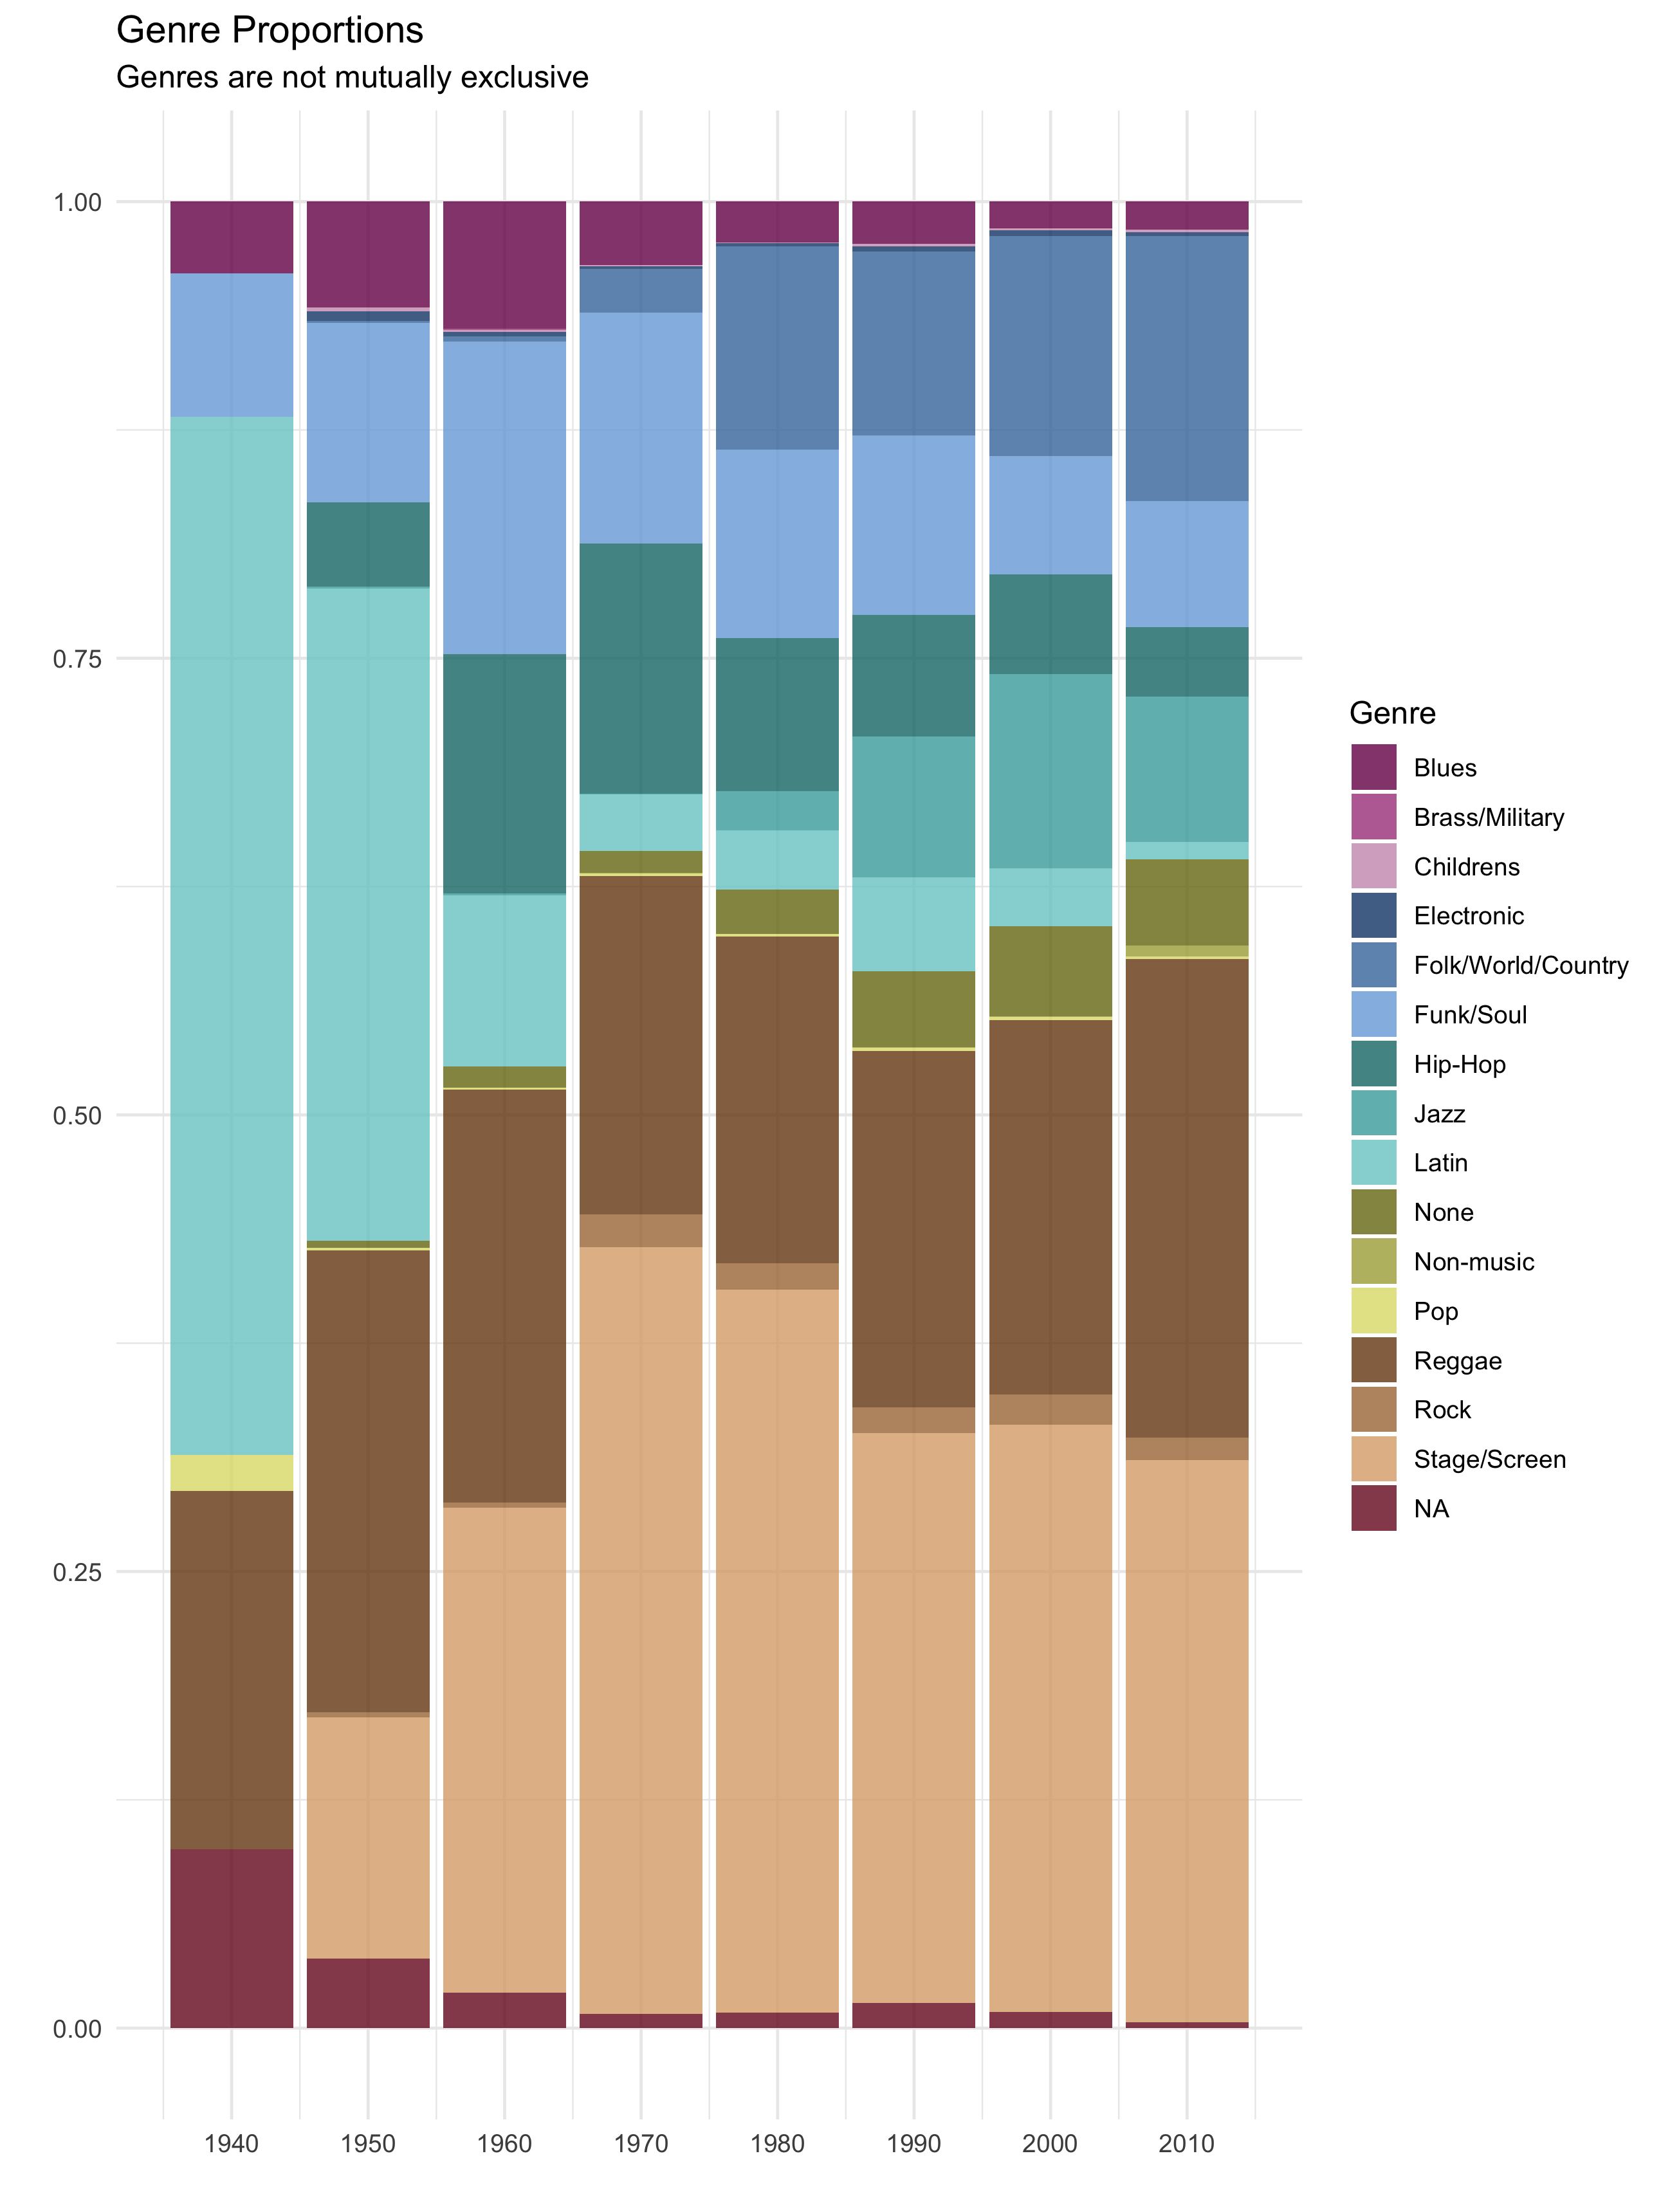
\includegraphics[width=6.5in]{genre_decade.png}
\end{center}
\subsection{Data Cleaning}
We used the \texttt{tidyverse} and \texttt{qdapTools} R libraries for data cleaning and munging. To prepare the data for analysis, we performed following data cleaning steps:  

\begin{itemize}
    \item Scraped lyrics data and meta data was cleaned of punctuation, newline characters, character return characters, and any HTML tags.
    \item Omitted any songs with no lyrics from analysis.
    \item Omitted any remixes, live renditions, re-releases.
    \item Dropped any duplicate songs using the song page url. Some songs are listed multiple times on Lyrics.com, but have the same url.
    \item Songs are tagged with genres and styles. We one-hot encoded all of these attributes. Our dataset includes 15 unique genres (including no genre), and 388 unique styles (also including no style).
    \item We used stop word dictionaries from the \texttt{tidytext} and \texttt{tm} libaries to remove stop words for the following languages: English, Espa\~{n}ol, Fran\c{c}ais, Portug\^{u}es, and Italiano.
    \item Omitted words that are solely comprised of punctuation characters.
    \item Omitted words that contain any numerics unless they are solely a one character length numeric i.e. 0-9. This is to account for the occurrences of meta-text in the song lyrics, e.g. "repeat x9"
\end{itemize}

After cleaning, our sample was reduced to 76,186 unique songs, which produced a corpus of 140,812 unique words. The below table shows the top 10 artists represented in our data.

\begin{center}
\begin{tabular}{|lc|lc|}
\hline
\textbf{Artist} & \textbf{n}\\
\hline
Elvis Presley & 408\\
\hline
Frank Sinatra & 358\\
\hline
Bing Crosby & 292\\
\hline
Ella Fitzgerald & 280\\
\hline
Dean Martin & 222\\
\hline
The Beatles & 210\\
\hline
Nat King Cole & 209\\
\hline
Johnny Cash & 206\\
\hline
Willie Nelson & 201\\
\hline
George Jones & 194\\
\hline
\end{tabular}
\end{center}

\section{Results}
Our main results can be summarized by the models' ability to predict genre. We used several model performance metrics to evaluate model predictive power, the first being AUC on a withheld set of test songs. On the next page, we plot test AUC by genre and the number of topics used to fit the LDA model.

For most genres, our LDA-derived features don't do a particularly great job of discriminating between songs in the genre and songs not in the genre. They do a particularly poor job on electronic music, a genre which tends to be lyrically sparser than the other genres. But on two genres, hip-hop and Latin music, the LDA-derived features do a very good job of classifying songs: test AUC is around 0.9 for all hip-hop classifiers and around 0.95 for all Latin classifiers. It may not be particularly surprising that it would do well on those two genres specifically: the hip-hop lexicon is highly distinctive, deriving heavily from African-American vernacular English, while Latin songs are heavy on words from different languages entirely. 

\begin{center}
    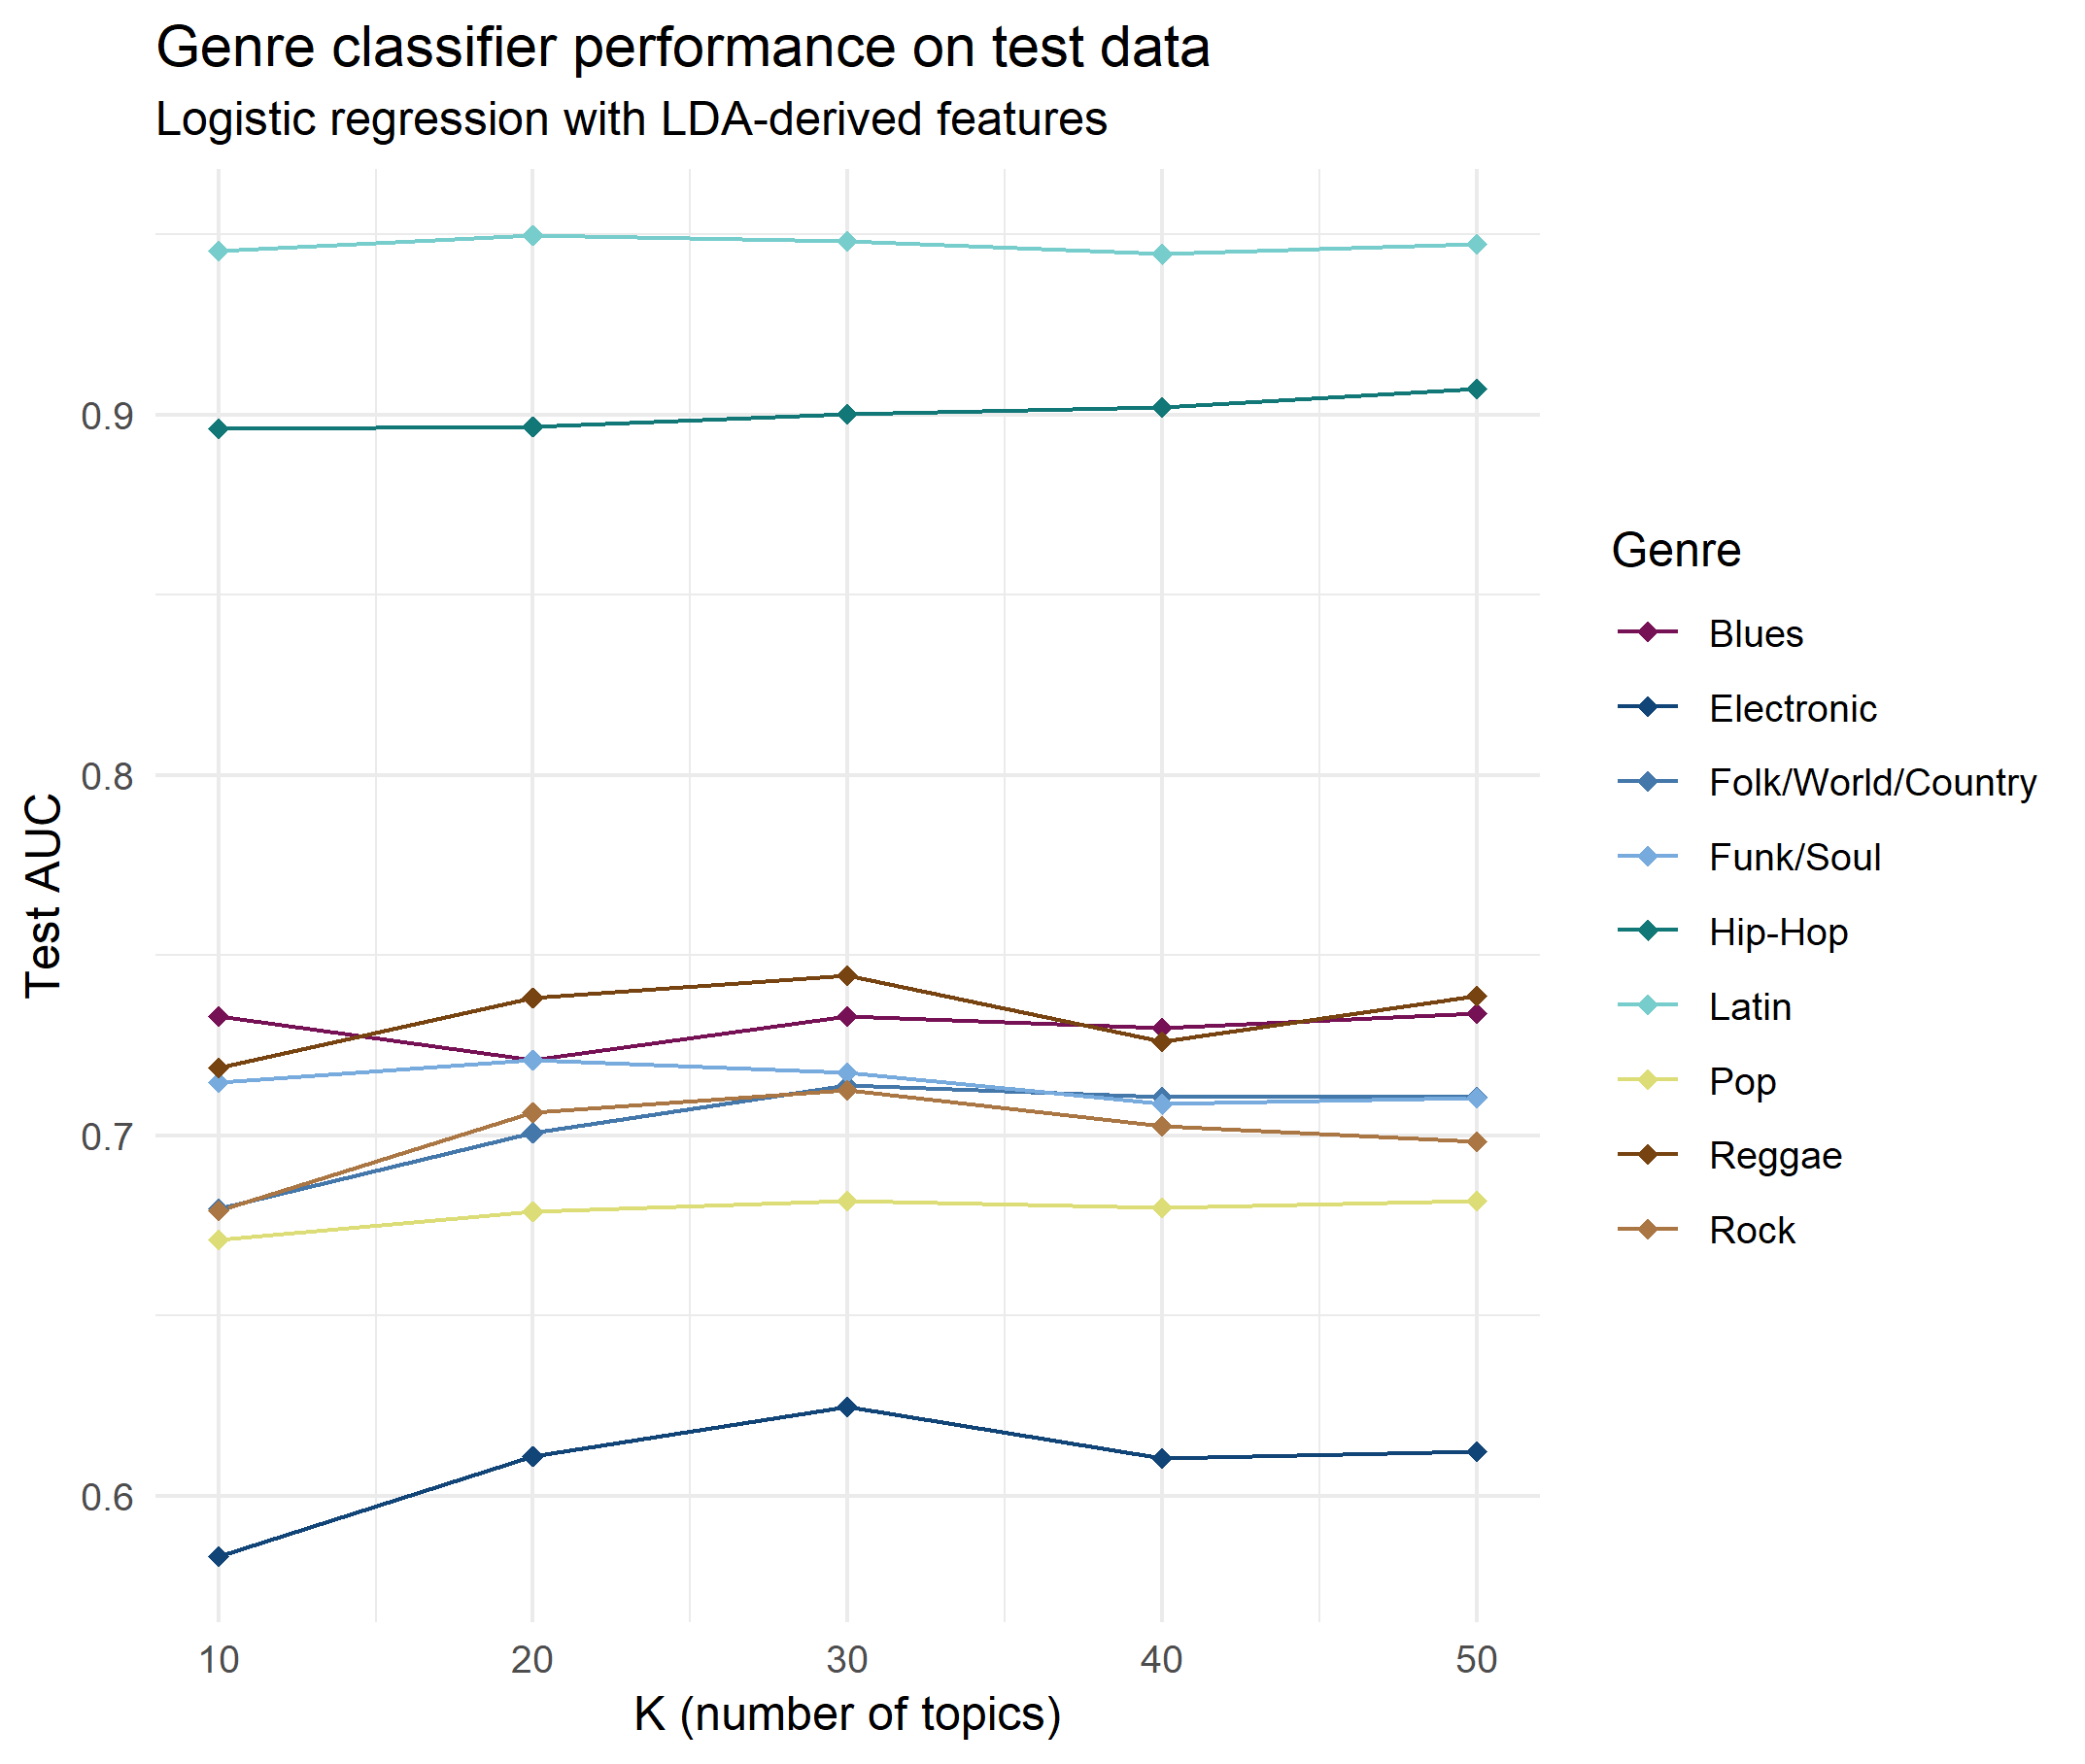
\includegraphics[width=6.4in]{model_aucs.png}
\end{center}

It also appears that increasing the number of topics or features doesn't have a significant effect on test AUC for most genres. Most genres seem to have a slight peak at $K=30$, so we also plot the ROC curves generated by the logistic regression models with 30 features.

\begin{center}
    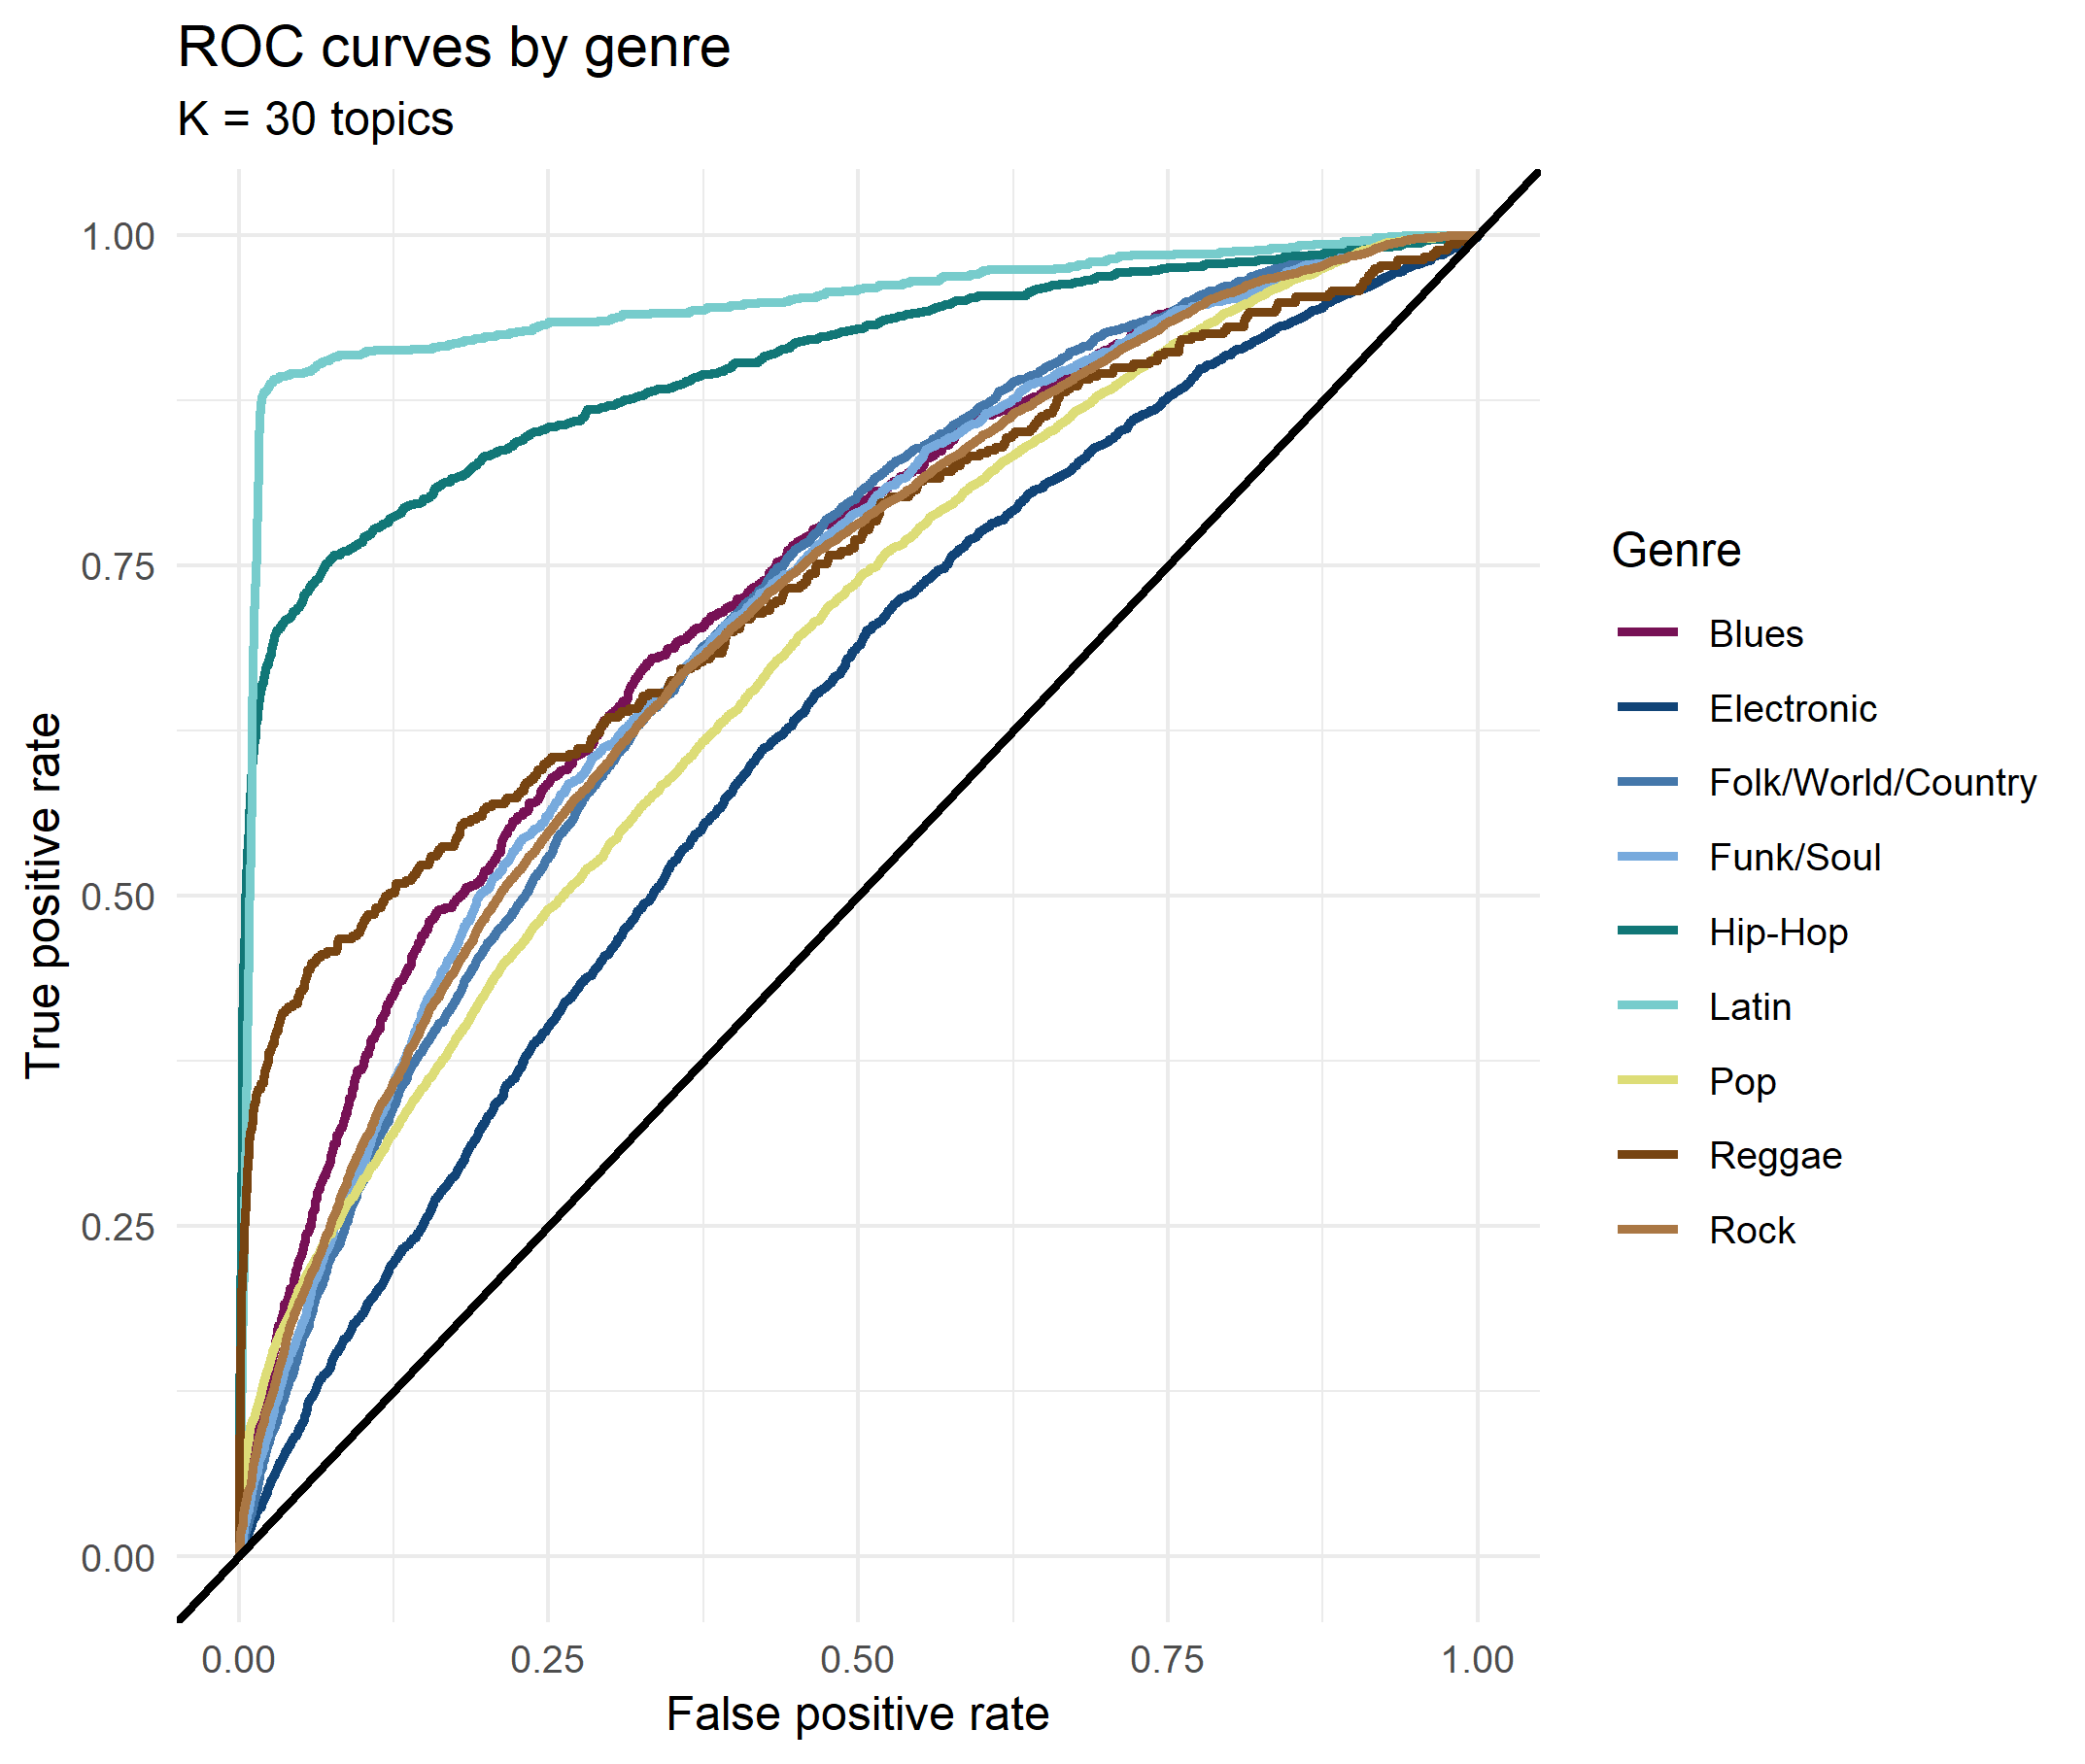
\includegraphics[width=6.4in]{roc_curves_k30.png}
\end{center}

However, we believe that in our context, where genre, in a qualitative sense, is not actually a binary outcome and in fact songs may belong to more than one genre, model calibration may be just as important as the model's ability to discriminate between positive and negative outcomes for each genre. Below, we have plotted the empirical and predicted probabilities of a song being in each genre in the 30-topic model, with bubble sizes corresponding to the proportion of songs that were predicted to be in-genre for each probability bin. 

\begin{center}
    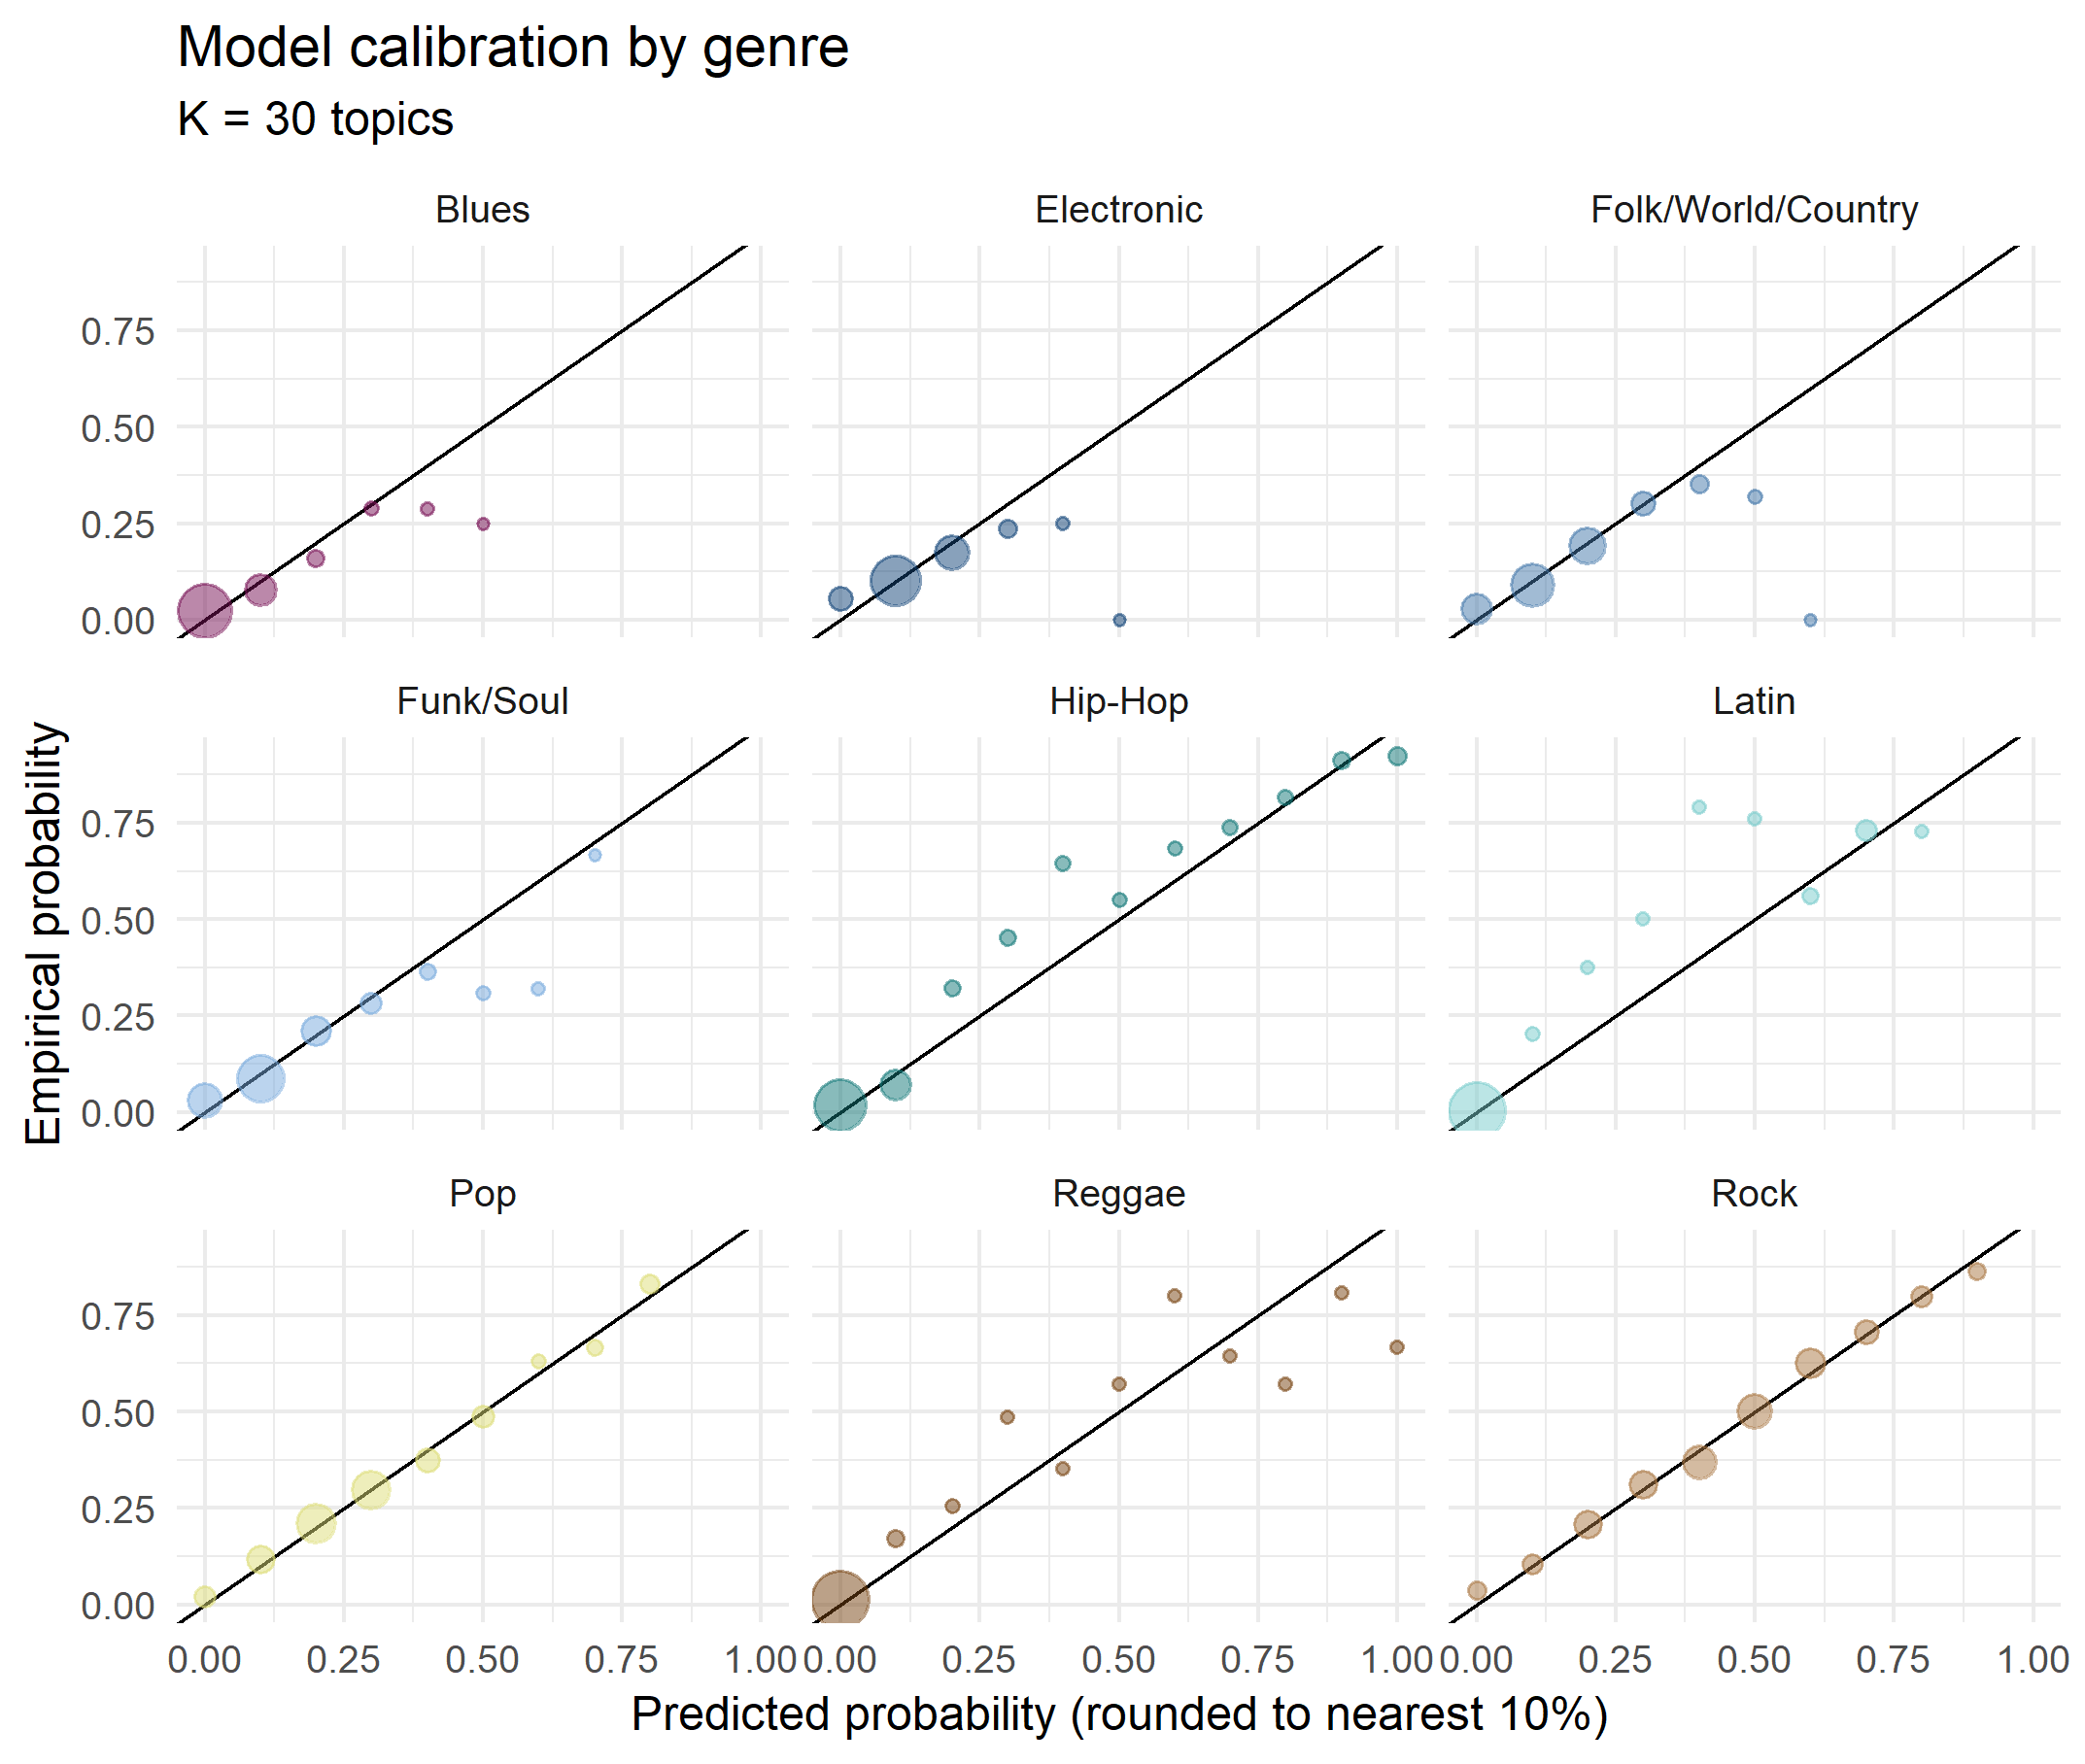
\includegraphics[width=6.4in]{calibration_k30.png}
\end{center}

In fact, when it comes to model calibration, it's for rock and pop songs that predicted probabilities best correspond to empirical probabilities of belonging to those genres, given how tightly the groups hug the 45-degree line in the rock and pop plots. The classifiers for the blues, electronic, and folk, world, and country genres were the least well calibrated, being overconfident in their predictions around the 50\% probability range. 

\section{Discussion}
Our model performance evaluations show that, overall, the LDA-derived features aren't particularly amazing at classifying songs into their respective genres, but their performance varies widely across genres. They are very good at classifying songs as hip-hop and Latin music, and particularly poor at classifying songs as electronic or not. Again, this trend isn't particularly surprising, given that the former two draw on highly distinctive lexicons, and the latter tends to draw on a smaller vocabulary than the other genres do. When it comes to model calibration, the predictions for whether songs fit into the rock and pop genres best correspond to the empirical probabilities at which they do so. 

The discrepancy appears to come specifically from the fact that hip-hop and Latin songs have those highly distinctive vocabularies, which mean that any song that lacks those words---and most of the songs in our sample do---will be classified as hip-hop or Latin with very low probability. As a result, it's possible to achieve extremely high sensitivity even for very low classification thresholds. By contrast, the rock and pop genres were large and lacked a particularly distinctive vocabulary, which may have contributed to the models' good calibration on those genres.

While these model evaluation plots tell us that the topics recovered by the LDA models are highly predictive of some genres and not particularly predictive for others, they don't tell us whether each individual topic recovered corresponds neatly to a particular genre. To determine this, we took within-genre means of the posterior probabilities for each topic and compared within topics across genres, the results of which are plotted on the following page.

Topics which correspond mostly to one genre will stand out in this plot as clearly unimodal distributions, with one genre dominating all others in that topic. In topic 6, for example, the dominant genre is clearly Latin music, and in topic 9 it's hip-hop. Topic 14 largely corresponds to reggae music, and topic 27 also appears to be a largely Latin music-related topic. As a sanity check, we can inspect the most frequently used words by topic (page after next).

\begin{center}
    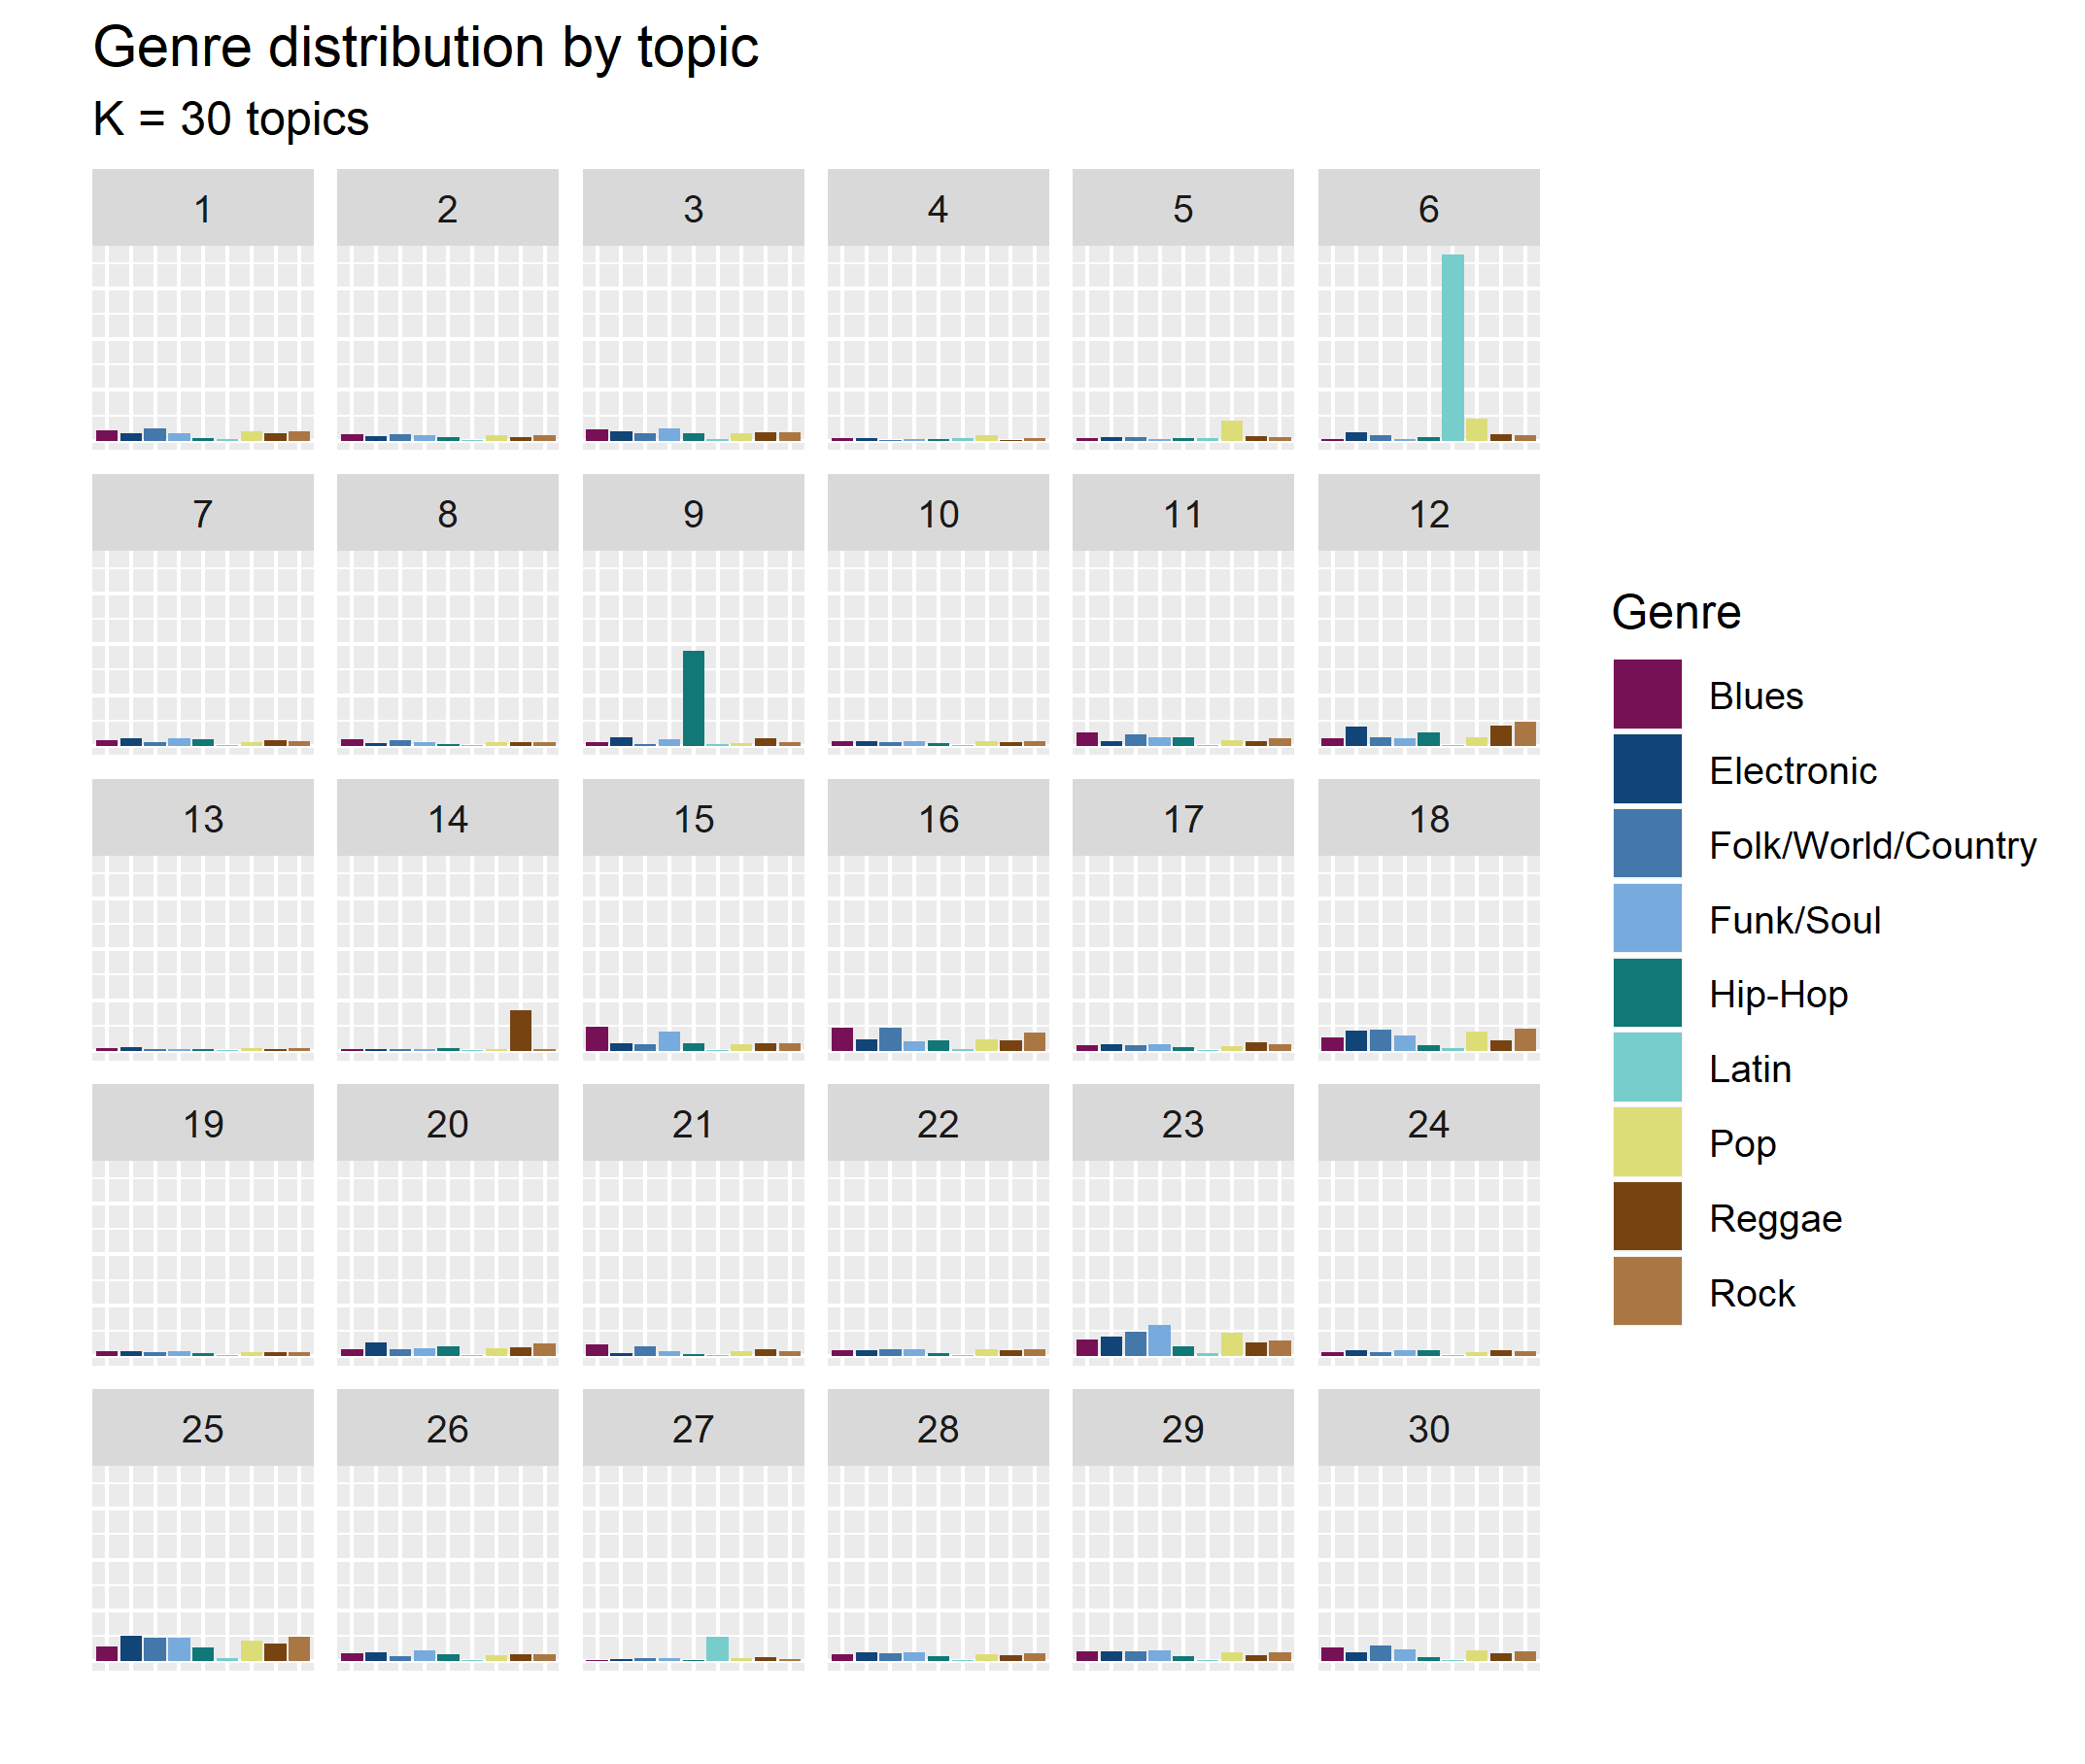
\includegraphics[width=7in]{genre_topic_distribution.png}
\end{center}

\begin{center}
    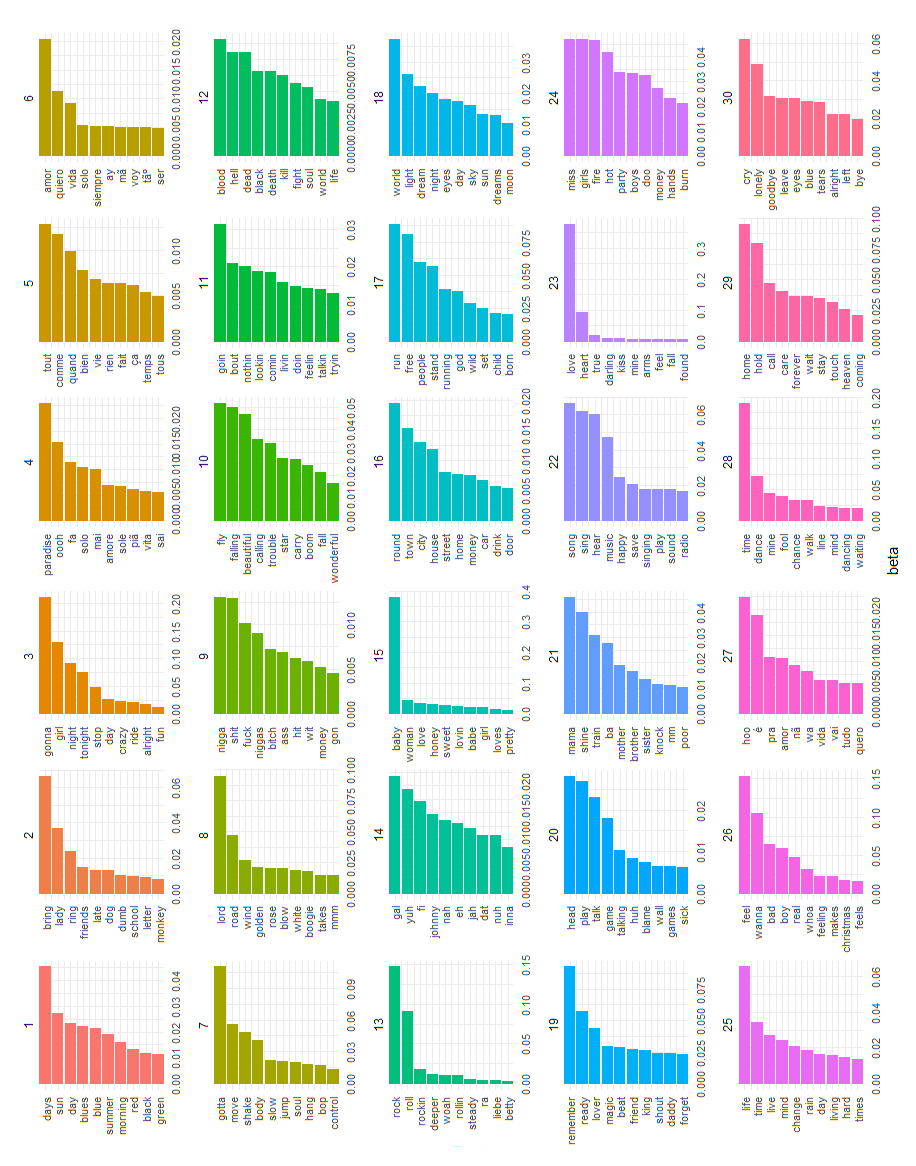
\includegraphics[width=7in]{k30_words.png}
\end{center}

The results corroborate what we saw in the previous within-topic genre distributions. Topic 6 is dominated by Spanish words; topic 9 is heavy on the kinds of swears and African-American vernacular most commonly found in rap music; topic 14 contains many words and vocalisms peculiar to reggae; and topic 27 also contains some Spanish words alongside Italian.

Other than those relatively extreme examples, however, for the most part the topics recovered by the 30-topic model don't really correspond to particular genres. By inspecting the words most likely to be generated by each topic, we can discern commonalities within topics, and more often than not those commonalities correspond to topics rather than genres---for example, topic 3 appears to be a topic about partying, topic 22 a topic about music and singing, topic 23 a song about romantic love, and so on. 

\section{Conclusion}
There are both internal and external validity issues. First, all content on Lyrics.com is user submitted without any rigorous quality control. Some songs were tagged with indisputably wrong genres according to expert opinion. Additionally, there is considerable noise in the style metadata. Style appears to attempt to be a sub-genre classification, but due to lack of quality control there are over 388 styles, and it's debatable how many of them should be considered sub-genres. There are also the types of internal validity issues that are expected from user submitted data such as missing attributes, typographical errors, multiple spellings for the same terms.

Our data may also have some external validity issues. The data used for analysis is not necessarily a representative sample of the entire song database on Lyrics.com. Additionally, songs are not balanced across countries, release years, or genres. We removed stopwords from multiple languages, but without considering what language the lyrics are actually from. For future work, the language of each song should be identified, and only stop words for that language removed. Furthermore, the use of lyric/song specific stop words should be considered. We considered 11 such words, however, future research should consider additional examination of the song lyrics corpus.

Finally, all LDA models were trained on the full lyrics corpus, instead of doing a train/test split, which is likely how a similar LDA model would be applied for a lyric classification task in practice. We attempted to split the input document-term-matrix into training and test sets that matched the songs in the training and test sets for the logistic models, but it wasn't clear to us how to split a \texttt{tidytext} document-term-matrix object while maintaining object fidelity.

Overall, the ability of the LDA-derived features to recover genre information appears to be spotty, being successful at lyric classification for only two genres out of the nine we examined. Apart from a few genres that draw on very distinctive lexicons, the topics recovered by LDA correspond more to actual song topics in the semantic sense rather than to existing genres generally agreed on by musicologists. This finding suggests that, if lyrics contribute a substantial part of musical experience for the deaf, then the generally agreed upon musical genres may have different meanings and relations to music lovers in the deaf community as compared to their meanings and relations to non-deaf people.

Further analysis should consider sentiment analysis of the topics derived in an attempt to uncover new definitions of musical genres that are solely lyric based, and may be more relevant to the deaf community. Additionally, we can consider fitting correlated topic models which also estimate a correlation between topics within documents. This could derive more predictive features because correlated topics may more closely match the non-exclusive membership of genres in our lyrics corpus. Also, other classification methods such as random forest or K-nearest neighbors could be used with the LDA-derived features for genre classification. The performance of all of these methods can be compared. Finally, more data should be scraped, and lyrical language should be identified through some other means so that language specific stop words can be removed in a more sophisticated manner. 

\bibliographystyle{unsrt}
\bibliography{bibliography}

\end{document}
